\documentclass[%
reprint,
%singlecolumn,
superscriptaddress,
%groupedaddress,
%unsortedaddress,
%runinaddress,
%frontmatterverbose, 
%preprint,
%showpacs,preprintnumbers,
%nofootinbib,
%nobibnotes,
%bibnotes,
%pre, 
floatfix,
amsmath,
amssymb,
aps,
notitlepage
]{revtex4-1}
%\usepackage[sort&compress,comma,numbers,round]{natbib}
\usepackage{graphicx}
\usepackage{bm}
\usepackage[hidelinks=true]{hyperref} 
\usepackage{xcolor}
\usepackage[hidelinks=true]{hyperref}
\usepackage{xcolor}
%\definecolor{greenish}{rgb}{0.13,0.58,0.16}
\definecolor{greenish}{RGB}{141,198,63}
\definecolor{reddish}{RGB}{239,65,54}
\definecolor{blueish}{RGB}{28,117,188}

\hypersetup{
colorlinks   = true, %Colours links instead of ugly boxes
urlcolor     = blueish, %Colour for external hyperlinks
linkcolor    = magenta, %Colour of internal links
citecolor   = greenish %Colour of citations
}
% \documentclass[12pt]{article}
% \usepackage{amsmath}
% \usepackage{amsfonts}
% \usepackage{amssymb,graphicx,fullpage}
\usepackage{mathrsfs}
\usepackage{bm}
\usepackage[hidelinks=true]{hyperref} 
\usepackage{xcolor}
\usepackage{mathrsfs}
\usepackage{bm, amsbsy}

\def\grad{\nabla}
\def\at{\hat{a}}
\def\Ai{\mathcal{A}}
\def\H{\mathcal{H}}
\def\J{\mathcal{J}}
\def\R{\mathbb{R}}
\def\d{\text{d}}
\def\e{\text{e}}
\def\r{\mathbf{r}}
\def\x{\mathbf{x}}
\def\xst{\mathbf{x}^*}
\def\u{\mathbf{u}}
\def\a{\mathbf{a}}
\def\T{\mathsf{T}}
\def\R{\mathbb{R}}
\def\E{\mathbb{E}}
\def\S{\mathcal{S}}
\def\pol{\pi_\theta}
\def\qsa{Q (s, a)}
\def\paa{\pi(a, s)}
\def\H{\sigma}
\def\grad{\nabla}
\def\th{\hat{\mathbf{t}}}
\def\ph{\hat{\mathbf{p}}}
\def\nh{\hat{\mathbf{n}}}
\def\yd{\dot{y}}
\def\ite{\text{ite}}
\def\P{\mathcal{P}}
\def\D{\mathcal{D}}
\def\Z{\mathcal{Z}}
\def\ah{\hat{a}}
\def\theta{\vartheta}
\def\H{\mathcal{H}}
\DeclareMathOperator*{\argmax}{arg\,max}
\def\OU{\rm OU}
\def\intP{\rm int}
\def\ebh{\hat{\mathbf{e}}}
\def\Pe{\mathsf{Pe}}

\begin{document}
\title{Dynamics of innovation in stigmergic collectives}
\author{S Ganga Prasath}
\email{sgangaprasath@iitm.ac.in}
\affiliation{Department of Applied Mechanics, Indian Institute of Technology Madras, Chennai TN 600 036.}
\date{}

\begin{abstract}
For later...
\end{abstract}

%\pacs{Valid PACS appear here}
\maketitle
Collectives in the wild often have to come up with novel solutions to problems either because
of uncertainties in the environment that demand new solution or due to high demands in the colony that
introduces a pressure to innovate. Ants, for egs., use stigmergy to recruit more
foragers to an identified food source by laying down pheromone along the trajectory they have taken towards the food source.
Even with pre-treaded paths in place, agents still have to explore to find
better solutions towards the food source if the demands of the colony are not met.
In this article, we probe the question of when and how collectives can innovate to find novel solutions
trajectories for foraging using stigmergy.

\section{Problem setting}
Social insects such as ants communicate either through pheromone or by antennation. Let us consider a trail of pheromone $\x^*(s)$ representing the position in 2-D coordinates and parameterized by the
arc-length $s$. The concentration of pheromone is considered continuous along this curve and is given by $c(\x) = c_o \delta(\x-\x^*(s))$.
This field is of course steady and its dynamics will be considered later in the article. The state of the agent/ant in
the environment is is represented by its position $\r^t=\{ r_x^t, r_y^t \}$ and the action it can take is to choose the
direction of motion i.e., its orientation $\ph^t = \{\cos(\theta^t), \sin(\theta^t)\}$, where $[\bullet]^t$ denotes the
value of the variable at time-instant $t$. The agent chooses its action based on the measurement at each time instant
which in this case is the concentration of pheromone, $c(\x)$.

\begin{figure*}
    \centering
    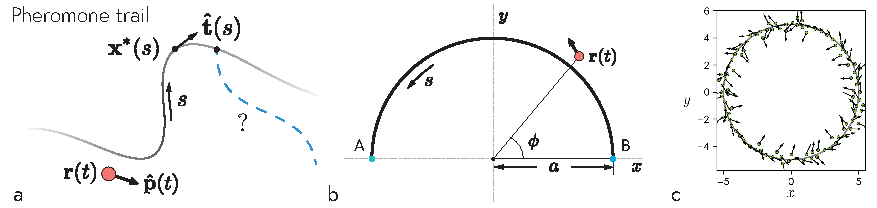
\includegraphics[width=\textwidth]{./figs/schematic.pdf}\label{fig:schm1}
    \caption{Schematic of setup}
\end{figure*}

\subsection*{Trail following behavior for semi-circular trail}

We know that stigmergy is one of the fundamental mechanisms by which the collective coordinates
and recruits new workers. With that being the case, the agent can follow the trail $\x^*(s)$ by making
measurements along its motion trajectory. Since we are interested in understanding how and when an
agent can innovate from its innate behavior of following pheromone trails to explore the environment and find novel solutions
to the navigation problem, we assume that the agent has already traversed the trajectory $\x^*(s)$ before.
This intrinsic behavior is denoted by the policy $\pi_{\rm int}(\r)$ which provides the
appropriate angle $\theta^t$ required to follow the trail when the agent is at location
$\r^t$ after the measurment that the agent makes. We consider the trail to be a simple semi-circle
with functional form $\xst(s) = \{ a \cos(s/a), a \sin(s/a) \}$ (see Fig.~\ref{fig:schm1}$(b)$). For this particular case,
the intrinsic trail following policy can be explicitly written as
\begin{align}
    \text{Measurement: } \phi^{t} = & \ \tan^{-1} \bigg( \frac{r_y^t}{r_x^t} \bigg) + \zeta^t, \\
    \text{Action: }\theta^{t} =& \ \frac{\pi}{2} + \phi^{t}, \\
    \text{State update: } \r^{t+1} =& \ \r^t + l \ph^{t}.
\end{align}
where $\zeta^t$ is the noise/error in the agent's measurement, $l$ is the step-length
of the agent. In the limit when the step-length is small, we can write the continuous version
of the motion as $\dot{\r} = v_o \ph$. Without loss of generality, we can write this as
$\d\r/\d s = \ph$ where $s = v_o t$. Moreover when the orientation of the agent
along its trajectory is distributed as though it were a worm-like chain polymer,
the functional form of orientation distribution is
\[
    \P[\theta(s)] = \frac{1}{\mathcal{Z}}\exp{(-\beta E_b)},
\]
where we define a bending energy for the trajectory captured by the agent's orientation as $E_b[\theta(s)]~=~B/2 \int_0^{s_c} (\theta'(s)-\kappa_o)^2~\d s$, the partition
function $\mathcal{Z}~=~\int \mathcal{D}[\theta(s)] \exp\{ {-\beta E_b[\theta(s)]} \}$ and the bending
stiffness $B$ captures the constraint for the agent to move forward towards the target A (ref Fig.~\ref{fig:schm1}$(b)$), $\beta$ is the effective
temperature capturing the fluctuations in the trajectory of agent. We also have
boundary conditions $\theta(0) = \pi/2$ (due to initial orientation of the agent) and $\theta'(0) = \kappa_o = a^{-1}$ (due to curvature of the trail).
Here $s_c$ is the coordinate along the semi-circle at which the agent bifurcates towards the target location A using a new trajectory.
Our motivation is to identify this location using the Bellman equation which will be discussed later.
Now in order to evaluate the quality of the intrinsic policy we introduce the notion of value function
of this policy $\pi_{\rm int}(\r)$, denoted by $v_{\rm int}(\r)$. The value function provides the cummulative
future reward that the agent will acquire from location $\r$ at time $t$
when following the policy $\pi_{\rm int}(\r)$. This can be written as
\[
    v_{\rm int}(\r) = \E_\pi \bigg[ \sum_{k=0}^\infty \gamma^k R_{t+k+1} \bigg| \r_t = \r \bigg].
\]
We can write this in path-integral form as (with $\gamma = 1$)
\begin{align}
    v_{\rm int}(\r) =& \ \sum_{k=t}^T \int \D[\theta(s)] \P[\theta(s)] \gamma^{k-t} R_{k+1}, \\
    \approx& \ \int_{s}^{s_c} \int \D[\theta(s)] \P[\theta(s)] R(s) \ \d s
\end{align}
The reward itself is a function of the agent's azimuthal direction, $\phi(s) = \tan^{-1}(y(s)/x(s))$.
Assuming that the reward has the function form $R(\phi) = \exp(-\phi/\phi^*)$, the leading order form of 
the value function for this policy is
\[
    v_{\rm int}(\r) = \frac{\phi^*}{\kappa_o} [ \e^{-\kappa_o s/\phi^*} - \e^{-\kappa_o s_c/\phi^*}].
\]

\subsection*{Search strategy post bifurcation}
After the agent leaves the trail trajectory at $\r(s_c)$, the agent needs to reach the target A.
Though the agent can take a variety of exploration strategies, we assume that the policy resembles
an Ornstein-Uhlenbeck (OU) process in the agent's orientation. This fits well with the behavior of an insect such as an ant because
ants often explore using their orientaiton after making measurements with their antennae.
This explorative policy $\pi_{\OU}(\r)$ can be written through $\P(\theta, t)$
the probability that the agent will take a particular angle $\theta$ at time $t$ or equivalently at distance $s$.
However, since the orientation of the agent is dependent on $\r(s_c)$, the angle between agent location $\r(s_c)$
to target A can be denoted as $\phi$ and $\theta=\phi+\varphi$ where $\varphi$ is the fluctuation around this
orientation that follows an OU-process. The probability $\P(\varphi, s)$ can then be written as
\[
    \frac{\partial \P}{\partial s} = \frac{\nu}{v_o} \frac{\partial(\varphi \P)}{\partial \varphi }
    + \frac{D}{v_o} \frac{\partial^2 \P}{\partial \varphi^2}
\]
where $\nu$ is the time-scale associated with relaxation of the agent's orientation to the target $\phi$
and $D$ represents the fluctuation in orientation, which we will soon assume to be large when $\r(s_c)$
is farther from the target A. Often in navigating insects, agents can quickly detect food source when they
are close to the food source. We capture this by assuming that after reaching a distance $\sigma$ from the end-point A,
agents can reach the target and thus the reward is a function only of the variance in agent's position towards the
target. Instead of solving the partial differential equation for $\P(\varphi, s)$, we can evaluate the
evolution of the variance of agent's position $\r(s)$ as it marches close to the target. Let $\ebh_\phi$
denote the orientation of the agent from $\r(s_c)$ to the target A. We can write the evolution of the variance
along $\ebh_\perp$ i.e. $\psi(s)=\E[r^2_\perp(s)]$ as $\d{\psi}(s)/\d s = 2 \E [ r_\perp(s) \varphi ]$ for $s>s_c$.
We can evaluate this evolution to get
\begin{align}
    \psi(s) - \psi(s_c) & = \frac{v_o^2 D}{\nu^3} \bigg[ \frac{2 \nu (s-s_c)}{v_o} - \e^{-2 \nu (s-s_c)/v_o} \nonumber \\
    & \ + 4 \e^{-\nu (s-s_c)/v_o} - 3 \bigg].
\end{align}
Before we move further with the calculation, it is cogent to work in non-dimensional numbers. In the OU-process
we have two length-scales: $l \sim (v_o/\nu), (v_o/D)$, one due to \textit{inertia} and other due to \textit{diffusion}.
The ratio of these two is nothing but the Peclet number, $\Pe = (D/\nu)$. We choose $l_\nu = (v_o/\nu)$ as the length-scale
for further non-dimensionalization such that $s \rightarrow l_\nu \hat{s}, t \rightarrow \nu^{-1} \hat{t}$. We drop the hat in what follows and we get
the non-dimensional variance, $\psi(s)$ (after setting $\psi(s_c) =0$) as a function of non-dimensional distance $s$ to be
\begin{align}
    \psi(s)& = \Pe \bigg[ 2 (s-s_c) - \e^{-2 (s-s_c)} + 4 \e^{-(s-s_c)} - 3 \bigg].
\end{align}
The non-dimensional Langevin dynamics that results in this evolution of the variance is $\d \varphi/\d s = - \varphi + \sqrt{2 \Pe} \eta(s)$.
As already mentioned, the agent reaching a distance $\sigma$ (appropriately non-dimensionalized with $l_\nu$) along $\ebh_\perp$ from the end-point A
can reach the target, then the probability that an agent will reach the target is given by $\P(||r_\perp^{s^*} - r^*|| \leq \sigma)
= \sigma/\psi(s^*)$. We can now calculate the value function, $v_{\rm OU}(\r, \theta)$ as
\[
    v_{\rm OU}(\r) = \int_{s_c}^{s^*} \int \D[\theta(s)] \P_{\rm OU}[\theta(s)] R(s) \ \d s.
\]
The reward function for the OU process takes a simple form $R(s) = \mu[1 - \Theta(||r_\perp(s^*) - r^*|| - \sigma)]$,
which simply means that the agent reaching within a distance $\sigma$ gets a reward $\mu$.
From this we see that the value function from $\r$ to the end of the trajectory, $v_{\rm OU}(\r^c) = \sigma \mu/\psi(s^*)$.

\section*{Value function of combined policy}
The total value function for the agent's policy is simply $v(\r, \theta) = v_{\rm int}(\r, \theta) + v_{\rm OU}(\r^c, \theta^c)$.
The agent is trying to maximize this value function from a given state, $\r^t, \theta^t$. The final expression
for the value function is
\[
    v(\r; s_c, D) = \frac{\sigma \mu}{\psi(s^*; s_c, \Pe)} + \frac{\phi^*}{\kappa} [ \e^{-\kappa s/\phi^*} - \e^{-\kappa s_c/\phi^*}],
\]
where we have introduced the non-dimensional number, $\kappa = \kappa_o l_\nu = (\kappa_o v_o/\nu)$.
In this equation, the Peclet number $\Pe$ captures the fluctuations in the dynamics of the agent
associated with the error in the homing vector. We assume that this diffusion is larger farther
from the target location and takes the functional form $\Pe \sim 1/s$. Moreover the reward that the agent recieves
when the bifurcation point is close to the target location needs to be smaller and thus $\mu = (\pi\kappa^{-1} -s_c)$.
One last detail that needs to be specified to make the value function complete is to specify $s^*$. It is straight
forward to show that from $s_c$, the target A is a distance $2 \cos(s_c\kappa/2)\kappa^{-1}$ which makes
$s^* = s_c + 2 \cos(s_c\kappa/2)\kappa^{-1}$.

\subsection*{Single agent learning}
Now that we have the environment and the agent behavior laid out, we look at the learning dynamics of the agent
when it has no feedback through pheromone but still tries to perform the distance-accuracy tradeoff. The agent can
make this tradeoff by exploring the environment as well as exploiting its intrinsic ability to follow pheromone to
accumulate reward. This is established through an $\epsilon$-greedy policy and we look at the evolution of the value
function as the agent so learns by following this strategy.

Mention that the TD(0)-learning results in
\[
    v(s_c) \leftarrow (1-\alpha) v(s_c) + \alpha r(s^*)
\]
as $v(s^*) = 0$.

%\sectionfont{\fontsize{15}{15}\selectfont}
%\subsectionfont{\fontsize{15}{15}\selectfont}
%\subsubsectionfont{\fontsize{15}{15}\selectfont}
\large
\widetext
\clearpage
\onecolumngrid
\begin{center}
\textbf{\large Supplemental Information for ``Dynamics of innovation in stigmergic collectives''}\\[.2cm]
S  Ganga  Prasath$^{1}$\\[.1cm]
{\small \itshape ${}^1$ Department of Applied Mechanics, Indian Institute of Technology Madras, Chennai TN 600 036.
}
\end{center}
%%%%%%%%% Merge with supplemental materials %%%%%%%%%%
%%%%%%%%% Prefix a "S" to all equations, figures, tables and reset the counter %%%%%%%%%%
\setcounter{equation}{0}
\setcounter{figure}{0}
\setcounter{table}{0}
\setcounter{page}{1}
\makeatletter
% \renewcommand{\theequation}{S\arabic{equation}}
% \renewcommand{\thefigure}{S\arabic{figure}}
% \renewcommand{\bibnumfmt}[1]{[S#1]}
%\renewcommand{\citenumfont}[1]{S#1}
%%%%%%%%% Prefix a "S" to all equations, figures, tables and reset the counter %%%%%%%%%%
\linespread{1.5}
% \setstretch{1.5}

%%%%%%%%% Prefix a "S" to all equations, figures, tables and reset the counter %%%%%%%%%%
%\renewcommand{\bibnumfmt}[1]{[S#1]}
%\renewcommand{\citenumfont}[1]{S#1}
%\renewcommand{\thesection}[1]{S#1\arabic{section}}
\renewcommand{\thetable}{S\arabic{table}}%
\renewcommand{\thesection}{S\arabic{section}}
%\renewcommand{\thesubsection}{SS\arabic{subsection}}
\renewcommand{\theequation}{S\arabic{equation}}
\renewcommand{\thefigure}{S\arabic{figure}}
%\renewcommand{\thesubsection}{SS\arabic{subsection}{}}
\renewcommand{\thesubsection}{\roman{subsection}{}}
%\renewcommand{\thesubsubsection}{(\roman{subsubsection}{})}

\subsection{Semi-circular trail}
For the problem at hand, we will considering a semi-circular trail whose coordinates can be
written in arc-length form as $\xst(s) = \{ a \cos(s/a), a \sin(s/a) \}$ where $a$ is the radius
of the circle. The trail starts at $s=0$ given by coordinates $\xst(0) = \{ a, 0 \}$ and ends at
$s=\pi a$ at $\xst (\pi a) = \{ -a, 0 \}$. From this it is easy to find that $\th(s) = \{ -\sin(s/a) , \cos(s/a) \}
= \{ \cos(\pi/2 + s/a), \sin(\pi/2 + s/a) \}$, and $\nh(s) = \{ -\cos(s/a) , \sin(s/a) \}$. We see that we
can represent $\th(s)$ through $\psi(s) = (\pi/2 + s/a)$. We can now calculate the location along the arc-length
where $\r(t)$ is closest by using the constraint condition $\d\r(t) \perp \th(s,t)$ or equivalently $\d\r(t)
\cdot \th(s,t) = 0$. We can now write $\d \r(t) \sim \{ a \cos(s/a) - r_x, a \sin(s/a) - r_y \}$
(up to normalization) and get the location $s_*(t) = a \tan^{-1}(r_y/r_x)$ by using the formula
for $\th(s)$. From this it is trivial to see that the angle along $\d \r$ is $\phi(t) = \tan^{-1}(r_y/r_x)$
(as is evident in Fig.~\ref{fig:schm1}$(b)$). For a given location of the agent, $\r(t)$ the orientation
it needs to take in the next step can be easily calculated to be $\theta(t) = (\pi/4 - \phi(t))$.

We can now set up the entire dynamics of the agent's trail following behavior on this semi-circle. We can state this
in the notation of reinforcement learning as it will become helpful later. The state of the agent
is $S^t = \{ r_x^t, r_y^t \}$, the measurements it makes are $M^t = \phi^t$ and using this information
the action the agent takes is $A^t = \{ \theta^t \}$ which is its orientation. The dynamics of
the agent can now be written as follows:
\begin{align}
    \text{Measurement update: } \phi^{t+1} = & \ \tan^{-1} \bigg( \frac{r_y^t}{r_x^t} \bigg) + \zeta^t, \\
    \text{Action update: }\ph^{t+1} =& \ \th^{t+1} + \d\r^{t+1}, \\
    \text{State update: } \r^{t+1} =& \ \r^t + l \ph^{t+1},
\end{align}
where $\r^t = \{ r_x^t, r_y^t \}$, $\d\r^t = (\xst(s^t)-\r^t)/||\xst(s^t)-\r(t)||$ and $\ph^t = \{ \cos \theta^t, \sin \theta^t \}$.
We have added sensory noise $\zeta^t$ (which is sampled from a uniform distribution) to the measurement
to reflect the error that accompanies measurements usually. The solution dynamics is shown
in Fig.~\ref{fig:schm1}$(c)$. We call this line-following behavior as a policy
$\pi_\ite(\r, \phi): $
which denotes the agent's innate behavior to follow pheromone trails.

\section{Ornstein-Uhlenbeck process}

Let us consider an agent whose orientation $\ph = ( \cos \theta, \sin \theta)$ wants to relax to a
neutral orientation with stochasticity associated with estimation error. The dynamics of the orientation
can be written as a stochastic differential equation given by
\begin{align}
    \dot{\theta}(t) =& \ - \alpha \theta(t) + \sqrt{2 D} \eta(t), \\
    \langle \eta(t) \eta(0) \rangle =& \ \delta(t).
\end{align}
This is the evolution of the famous Ornstein-Uhlenbeck process which has been extremely well studied
and the evolution of the probability density can be solved exactly. The Fokker-Planck equation for
its dynamics which provides the probability of a given state $\theta(t)$ i.e. $p(\theta, t)$, is given by
\[
    \frac{\partial \P}{\partial t} = \alpha \frac{\partial(\theta \P)}{\partial \theta }
    + D \frac{\partial^2 \P}{\partial \theta^2}
\]
The dynamics of the angle relaxes to equilibrium angle $\theta = 0$ in the absence of fluctuations.
The evolution of the mean is $\dot{h}(t) = - \alpha h(t)$ where $h(t) = \E [ \theta(t) ]$
while the co-variance dynamics is given by $\dot{\zeta}(t) = -2\alpha \zeta(t) + 2D$ with
$\zeta = \E [  {(\theta(t) - h(t))}^2 ] = \E [  \theta^2(t) ] - h{(t)}^2$.

The position of the agent evolves as $\dot{\r}(t) = v_o \ph(t)$. Under the assumption that the angle
is small, we can write $\dot{\r}(t) = v_o (1, \theta)$. Thus we have $\yd (t) = v_o \theta$ which can
be used to rewrite the orientation equation as
\begin{align}
    \ddot{y}(t) =& \ - \alpha \yd (t) + v_o\sqrt{2 D} \eta(t).
\end{align}
This second order equation needs to boundary condition. We require $y(0) = 0$ and $\yd (0) = 0$ which
comes from setting the initial orientation to be 0. We are interested in the evolution of the mean and
the variance of this SDE. Let $m(t)= \E [  y(t) ]$ where the averaging is the ensemble average
(equivalently the average of the several trajectories of the same dynamics). The mean $m(t)$ evolves as
\begin{align}
    \ddot{m}(t) =& \ -\alpha \dot{m}(t).
\end{align}
By applying the above boundary condition, we can immediately see that $m(t) = 0$. Nevertheless, we are
interested in the evolution of the standard deviation, $\beta(t) = \E [  {(y(t) - m(t))}^2 ]$.
In order to derive an expression for that, we differentiate the definition once to get
\begin{align*}
    \dot{\beta}(t) =& \ 2 \E [ \{ y(t) - m(t) \} \{ \yd(t) - \dot{m}(t) \} ], \\
    = & \ 2 \E [ y \yd ] - 2 m \dot{m}, \\
    = & \ 2 v_o \{ \E [ y \theta ] - m \dot{m}\}.
\end{align*}
We can estimate $\E [ y \theta ]$ as follows
\begin{align*}
    \E [ y \theta ] =& \ v_o \E \bigg[ \int_0^t \theta(s) \theta(t) \ \d s \bigg], \\
    =& \ v_o  \int_0^t \E [ \theta(t) \theta(s) ] \ \d s.
\end{align*}
We know that for an OU process, 
\[
    \E [ \theta(t) \theta(s) ] = \frac{D}{\alpha} \bigg[ \e^{-\alpha(t-s)}-\e^{-\alpha(t+s)} \bigg].
\]
From this we see that
\begin{align*}
    \E [ y \theta ] =& \ \frac{v_o D}{\alpha} \int_0^t  \bigg[ \e^{-\alpha(t-s)}-\e^{-\alpha(t+s)} \bigg] \ \d s, \\
    =& \ \frac{v_o D}{\alpha^2} \bigg[ 1 - 2 \e^{-\alpha t} + \e^{-2 \alpha t}\bigg].
\end{align*}
We thus have the evolution of the co-variance of $y(t)$ as
\begin{align}
    \dot{\beta}(t) = & \  \frac{2 v_o^2 D}{\alpha^2} \bigg[ 1 - 2 \e^{-\alpha t} + \e^{-2 \alpha t}\bigg].
\end{align}
We finally have the variance as a function of time as
\begin{align}
    \beta(t) & = \frac{v_o^2 D}{\alpha^3} \bigg[ 2 \alpha t - \e^{-2 \alpha t} + 4 \e^{-\alpha t} - 3 \bigg].
\end{align}
For $t \gg \alpha^{-1}$ we can immediately see that $\beta(t) \approx 2v_o^2 D t/\alpha^2$. We are interested
in the variance at time, $t^* = c/v_o$ where $c$ is the distance of the agent from the goal A and $v_o$
is the intrinsic speed of the agent. At this time the location of the agent along x-axis is $x(t^*)=c$
while the variance in $y(t)$ is $\beta(t^*) \approx 2v_o D c/\alpha^2$.
% Differentiating this once more, we get
% \begin{align*}
%     \ddot{\beta}(t) =& \ 2 [ v_o \langle (\yd \theta + y \dot{\theta} \rangle - \dot{m}^2 - m \ddot{m}]
% \end{align*}


\section{Evaluating value function of policies}
We are at a stage where we can solve the speed/distance-accuracy trade-off for the an agent trying
to make optimal decision on when to initiate innovation. In order to do that, let us define clearly
what is the state and action of the agent.
\subsection{$v(\r, \theta)$ for $\pi_{\rm int}(\r, \theta)$}
The agent's state $s^t$ is given by its position, $s^t: \r^t=\{ x^t, y^t \}$ and the action it can take
at these location is choose a orientation to move, $a^t: \theta^t$. Once the agent choose this action,
it is taken to the next state $s^t$ through the dynamics: $\r^{t+1} = \r^t + l \ph_\theta^{t}$.
Before we compute the state-value function for the intrinsic policy, $\pi_{\rm int}(s)$, the sequence
of process we described above can be written as
\begin{align}
    \text{Measurement: } \phi^{t} = & \ \tan^{-1} \bigg( \frac{r_y^t}{r_x^t} \bigg), \\
    \text{Action, $a^t$: }\theta^{t} =& \ \frac{\pi}{2} + \phi^{t} + \zeta^t, \\
    \text{State update, $s^{t+1}$: } \r^{t+1} =& \ \r^t + l \ph_\theta^{t}.
\end{align}
It is however difficult to evaluate the value function for this specific functional form of the policy.
We assume that the distribution of the orientation of the agent is distributed as through
it is a worm-like chain polymer whose orientation distribution is given by
\[
    \P[\theta(s)] = \frac{1}{\mathcal{Z}}\exp{(-\beta E_b)}
\]
where the bending energy $E_b[\theta(s)] = B/2 \int_0^L (\theta'(s)-\kappa_o)^2 \ \d s$, fugacity
$\mathcal{Z} = \int \mathcal{D}[\theta(s)] \exp\{ {-\beta E_b[\theta(s)]} \}$ and the bending
stiffness $B$ captures the constraint for the agent to move forward, $\beta$ is the effective
temperature capturing the fluctuations in the trajectory of agent. We also have
boundary conditions $\theta(0) = \pi/2$ and $\theta'(0) = \kappa_o = a^{-1}$. 

% We can discretize the bending energy as
% \[
%     E_b[\theta] = \frac{B}{2} \sum_0^n l \bigg( \frac{\theta^{n+1} - \theta^n}{l}  - \kappa_o \bigg)^2.
% \]
We are interested in evaluating the value function of this policy, $v(s^t)$ whose
expression is given by
\[
    v_{\rm int}(\r, \theta) = \E_\pi \bigg[ \sum_{k=0}^\infty \gamma^k R_{t+k+1} \bigg| S_t = S \bigg].
\]
We can write this in path-integral form as
\begin{align}
    v_{\rm int}(\r, \theta) =& \ \sum_{k=t}^T \int \D[\theta(s)] \P[\theta(s)] \gamma^{k-t} R_{k+1}, \\
    \approx& \ \int_{s}^L \int \D[\theta(s)] \P[\theta(s)] R(s) \ \d s
\end{align}
The reward itself is a function of the agent's azimuthal direction, $\phi(s) = \tan^{-1}(y(s)/x(s))$.
Further we know the geometric relation $x'(s) = \cos(\theta(s)), y'(s) = \sin(\theta(s))$. The functional
form of the reward is $R(\phi) = \exp(-\phi/\phi^*)$ and 
\[
    \phi(\r, \theta) = \tan^{-1}\bigg( \frac{\int_0^s \sin(\theta(\tau)) \ \d \tau}{\int_0^s \cos(\theta(\tau)) \ \d \tau} \bigg)
\]
We can write the ultimate expression for the value function we would like to evaluate as,
\begin{align}
    v_{\rm int}(\r, \theta) =& \ \int_{s}^L \int \D[\theta(s)] \P[\theta(s)] \exp(-\phi(s)/\phi^*) \ \d s'.
\end{align}
We know that $\theta(s)$ has to satisfy the boundary conditions $\theta(0) = \pi/2$ and $\theta'(0) = \kappa_o$.
Before we solve the stochastic version of the problem, let us solve it for the deterministic case when
the agent follows the semi-circular path exactly. In this scenario, $\theta_b(s) = \pi/2 + \kappa_o s$ and
from this it immediately follows that $\phi_b(s) = \kappa_o s$. For this particular functional form of $\phi(s)$
we can write the reward as $R(s) = \exp(-\kappa_o s/\phi^*)$. The value function from this can be written as
\begin{align}
    v_b(s) =& \ \int_s^L \exp(-\kappa_o \tau/\phi^*) \ \d \tau, \\
    =& \ -\frac{\phi^*}{\kappa_o} [\e^{-\kappa_o L/\phi^*} - \e^{-\kappa_o s/\phi^*}], \\
    =& \ \frac{\phi^*}{\kappa_o} \e^{-\kappa_o L/\phi^*} [ \e^{\kappa_o(L-s)/\phi^*} - 1].
\end{align}
We now introduce perturbations in the trajectory of the agent from the trajectory $\theta_b(s)$ by introducing
perturbations $\theta(s) = \theta_b(s) + \delta \theta(s)$. We know that $\phi$ and $\theta$ are related by the
geometric constraint: $\phi(s) = \theta(s) - \pi/2$ which immediately gives $\phi(s) = \kappa_o s + \delta \theta(s)$.
We can then write the value function as
\begin{align}
    v_{\rm int}(s) =& \ \int_{s}^L \int \frac{ \D[\theta(s)]}{\mathcal{Z}}\e^{-(\beta B/2) \int_0^L (\theta'(s)-\kappa_o)^2 \ \d s} \exp(-\phi(\tau)/\phi^*) \ \d \tau, \\
    =& \ \int_{s}^L \int \frac{ \D[\theta(s)]}{\mathcal{Z}}\e^{-(\beta B/2) \int_0^L [\delta \theta'(s)]^2 \ \d s} \e^{(-\kappa_o \tau - \delta \theta(\tau))/\phi^*} \ \d \tau.
\end{align}
Let us start by calculating $\Z$,
\begin{align}
    \Z =& \ \int \mathcal{D}[\theta(s)] \exp\{ {-\beta E_b[\theta(s)]} \}, \\
    =& \ \int \mathcal{D}[\theta(s)] \e^{-(\beta B/2) \int_0^L [\delta \theta'(s)]^2 \ \d s}, \\
    \delta \theta(s) =& \ \sum_{k=-\infty}^\infty \ah_k \e^{i 2 \pi k s/L}, \\
    \int_0^L [\delta \theta'(s)]^2 \ \d s =& \ \int_0^L \bigg[ \sum_{k=-\infty}^\infty \frac{2\pi k}{L} \ah_k i \e^{i 2 \pi k s/L} \bigg]
    \bigg[ \sum_{q=-\infty}^\infty \frac{2\pi q}{L} \ah_q i \e^{i 2 \pi q s/L} \bigg] \ \d s, \\
    =& \ \frac{4\pi^2}{L} \sum_{k=-\infty}^\infty k^2 \ah_k^2, \text{where we have used } \ah_{-k} = \ah_k \\
    \Z =& \ \prod_{k=-\infty}^\infty \int_{-\infty}^{\infty} \d \ah_k \e^{-\frac{\beta B k^2}{L} 4\pi^2\ah_k^2}, \\
    =& \ \prod_{k=-\infty}^\infty \sqrt{\frac{\pi L}{\beta B}} \frac{1}{2\pi k}
\end{align}
We can go ahead and write down the value function as
\begin{align}
    v_{\rm int}(s) =& \ \frac{1}{\Z} \prod_{k=-\infty}^\infty \int_{-\infty}^{\infty} \e^{-\frac{\beta B k^2}{L} 4\pi^2 \ah_k^2} \bigg[ \int_{s}^L \e^{(-\kappa_o \tau - \ah_k \e^{i 2 \pi k \tau/L})/\phi^*} \ \d \tau \bigg] \d \ah_k, \\
    =& \ \frac{1}{\Z} \prod_{k=-\infty}^\infty \int_{s}^L \bigg[ \int_{-\infty}^{\infty} \e^{-\frac{\beta B k^2}{L} 4\pi^2 \ah_k^2  - \ah_k \e^{i 2 \pi k \tau/L}/\phi^*} \ \d \ah_k \bigg]  \e^{-\kappa_o \tau/\phi^*} \ \d \tau.
\end{align}
We can evaluate the integral inside the square brackets as
\[
    \int_{-\infty}^\infty \e^{-\alpha \ah^2 -\gamma \ah} \ \d \ah = \e^{-\frac{\gamma^2}{4\alpha}}\int_{-\infty}^\infty \e^{-\alpha(\ah + \frac{\gamma}{2 \alpha})^2} \ \d \ah
    = \sqrt{\frac{\pi}{\alpha}} \e^{-\frac{\gamma^2}{4\alpha}}.
\]
We then get
\begin{align}
    v_{\rm int}(s) =& \ \sqrt{\frac{\pi L}{\beta B}}  \frac{1}{\Z} \prod_{k=-\infty}^\infty \frac{1}{2\pi k}  \int_{s}^L \e^{-\gamma(k, \tau)^2/4\alpha} \e^{-\kappa_o \tau/\phi^*} \ \d \tau.
\end{align}
where $\gamma(k, \tau) = \e^{i 2 \pi k \tau/L}/\phi^*, \alpha = \beta B k^2 4 \pi^2/L$. In the limit of small temperature,
or large bending stiffness, $\alpha \gg 1$ and we can Taylor expand the integral to get
\begin{align}
    v_{\rm int}(s) =& \ \sqrt{\frac{\pi L}{\beta B}}  \frac{1}{\Z} \prod_{k=-\infty}^\infty \frac{1}{2\pi k}  \int_{s}^L \bigg[ 1 - \frac{\gamma(k, \tau)^2}{4\alpha} \bigg] \e^{-\kappa_o \tau/\phi^*} \ \d \tau.
\end{align}
From this we see that the leading order contribution is still
\begin{align}
    v_{\rm int}(s) =& \ \frac{\phi^*}{\kappa_o} \e^{-\kappa_o L/\phi^*} [ \e^{\kappa_o(L-s)/\phi^*} - 1].
\end{align}

\subsection{$v(\r, \theta)$ for $\pi_{\rm OU}(\r, \theta)$}
We have seen already the dynamics of the OU process and we can write the policy $\pi_\text{OU}(\r, \theta)$ using the evolution
of the orientation and position as
\begin{align}
    \theta^{t+1} =& \ \theta^t (1 - \mu \Delta t ) + \sqrt{2 D \Delta t} \zeta^t, \\
    % \dot{\theta}(t) =& \ - \alpha \theta(t) + \sqrt{2 D} \zeta(t), \\
    \langle \zeta^t \zeta^0 \rangle =& \ \delta(t), \\
    \r^{t+1} =& \ \r^{t} + l \ph_\theta^t, \text{where} \ \ph_\theta^t = \{ \cos \theta^t, \sin \theta^t \}.
    % \dot{\r}(t) =& \ v_o \ph
\end{align}
We have calculated the evolution of variance of the agent's trajectory from a straight line as a function of
distance/time from the bifurcation point evolves as,
\begin{align}
    \psi(t) & = \frac{v_o^2 D}{\mu^3} \bigg[ 2 \mu t - \e^{-2 \mu t} + 4 \e^{-\mu t} - 3 \bigg].
\end{align}
where $\mu^{-1}$ is the time-scale of relaxation of the agent. The $n$-step variance of the agent is
$\psi (t^*)$, where $t^* = n \Delta t$. Assuming that the agent reaching a distance $\sigma$ from the end-point A can reach the
target, the probability that an agent will reach the target is given by $\P_{\rm OU}(||\r^{n\Delta t} - \r^*|| \leq \sigma)
= \sigma/\psi(t^*)$. We can now calculate the value function, $v_{\rm OU}(\r, \theta)$ using the formula
\[
    v_{\rm OU}(\r, \theta) = \int_{0}^{t^*} \int \D[\theta(t)] \P_{\rm OU}[\theta(t)] R(t) \ \d t.
\]
Let us assume that the reward function for the OU process is $R(t) = \nu[1 - \Theta(||\r(t^*) - \r^*|| - \sigma)]$.
From this we see that the value of $v_{\rm OU}(\r^c, \theta^c) = \sigma \nu/\psi(t^*)$.

\section{Value function of combined policy}
The total value function for the agent's policy is $v(\r, \theta) = v_{\rm int}(\r, \theta) + v_{\rm OU}(\r^c, \theta^c)$.
The agent is trying to maximize this value function from a given state, $\r^t, \theta^t$. The final expression
for the value function is
\[
    v(\r, \theta) = \frac{\sigma \nu}{\psi(t^*+t_f)} + \frac{\phi^*}{\kappa_o} \e^{-\kappa_o s^*/\phi^*} [ \e^{\kappa_o(s^*-s)/\phi^*} - 1],
\]
where $\psi(t) = \dfrac{v_o^2 D}{\mu^3} \bigg[ 2 \mu t - \e^{-2 \mu t} + 4 \e^{-\mu t} - 3 \bigg]$, $t_f$ is the time-taken to reach
the region around the target location A. In this equation, the diffusion coefficient
representing the fluctuations in the dynamics of the agent capturing the error in memory
of target location A. We assume that the fluctuation $D$ is larger farther from the target location.

% It is however difficult to evaluate the value function of this specific functional form of the policy.
% Instead we move to a different form given by the Langevin dynamics of the orientation satisfying
% the equation:
% \begin{align}
%     \gamma \partial_j \phi (s, j) =& \ B \partial_s^2 \phi (s, j) + \Gamma(s, j),
% \end{align}
% where the arc-length $s \in (0, L], L = nl$ and epoch $j = 0 \dots N$. The bending stiffness $B$
% in the equation captures the constraint that the motion of the agent is in the forward direction.
% Further this equation is subject to the boundary condition $\phi(0, j) = 0, \phi'(0, j) = \kappa_o$ with $\kappa_o$ being
% the curvature of the initial pheromone trail, $\kappa_o \sim a^{-1}$. Here $\Gamma(s, j)$ is the
% spatio-epochal delta-correlated noise whose variance is given by
% \[
% \langle \Gamma_\alpha \Gamma_\beta \rangle = 2 \gamma D \delta_{\alpha \beta} \delta(s-s') \delta(j-j')
% \]

% The interpretation of this equation is the the orientation dynamics of the agent undergoes a diffusion but the overall trajectory has 
% an intrinsic curvature (arising out of the boundary condition). Here $s$ is the arc-length which is
% equivalent to $k$-step motion of the agent i.e. $s_k = k l = k v_o \delta t$. Similarly $j$ in the
% equation is the $j$-th epoch of $k$-step trajectory of the agent. The location of the agent is given by
% $\partial_s \r(s,j) = \th_\theta(s, j) = \{ \cos \phi(s, j), \sin \phi(s, j) \} = \{ -\sin \theta(s, j), \cos \theta(s, j) \}$. Once we know $\phi(s, j)$
% can evaluate the position, $\r(s, j)$ and the orientation $\theta(s, j)$. In this framework
% the policy $\pi_{\rm int} (\r(s))$ for the $j$-th epoch gives the action $\phi(s)$ that moves the agent
% along using the geometric constraint/equation $\r'(s) = \th_\theta(s)$.
% \textbf{Don't need temporal/epochal dynamics}

\end{document}